\begin{frame}
\frametitle{Electric dipole moments (EDMs)}

\begin{columns}
\column{0.72\textwidth}
\vspace{-0.4cm}
 \begin{block}{For particles with EDM $\vec d$ and MDM $\vec \mu$ ($\propto \vec s $),}
 \begin{itemize}
     \item non-relativistic Hamiltonian:
        \begin{equation}
            H = -\vec \mu \cdot \vec B - \vec d \cdot \vec E \nonumber
        \end{equation}
 \item \textbf{Energy of magnetic dipole} invariant under $P$ and $T$:
 \begin{equation}
  -\vec \mu \cdot \vec B \overbrace{\longrightarrow}^{P \text{ or } T} -\vec \mu \cdot \vec B \nonumber
 \end{equation}
 No other direction than spin  $\Rightarrow$ $\vec d$ parallel to $\vec \mu$ ($\vec s$). 
  \item \textbf{Energy of electric dipole} $H = - \vec d \cdot \vec E$, includes term 
  \vspace{-0.2cm}
  \begin{equation}
  \vec s \cdot \vec E \overbrace{\longrightarrow}^{P \text{ or } T} - \vec s \cdot \vec E,
 \end{equation}
 % \end{itemize}
 \end{itemize}
 \end{block}
\column{0.27\textwidth}
\begin{figure}
	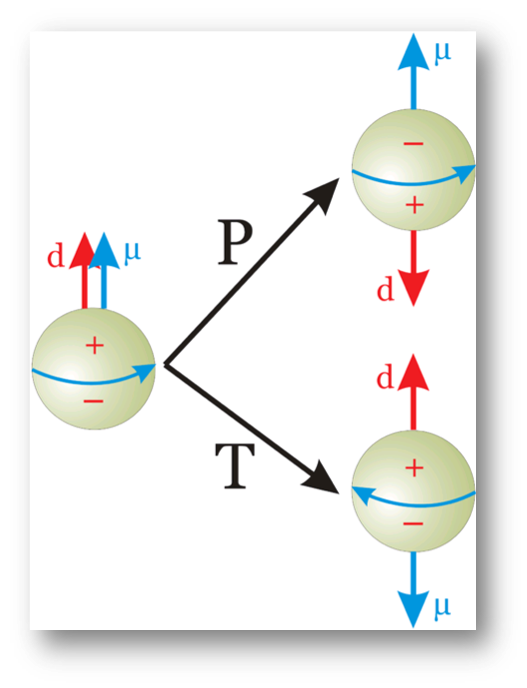
\includegraphics[width=1\textwidth]{EDM-graphic}
\end{figure}
\end{columns}
 

\begin{alertblock}{\textbf{EDMs violate both $P$ and $T$ symmetry}}
\begin{itemize}   
     \item EDMs possibly constitute the missing cornerstone to explain surplus of matter over antimatter in the Universe.
     \begin{itemize}
        \item Non-vanishing EDMs would add \nth{4} quantum number to fundamental particles (besides $m$, $q$, and $s$).  
     \end{itemize}
\end{itemize}
\end{alertblock}


%  \column{0.3\textwidth}
% \vspace{-0.2cm}
%     \begin{figure}
%       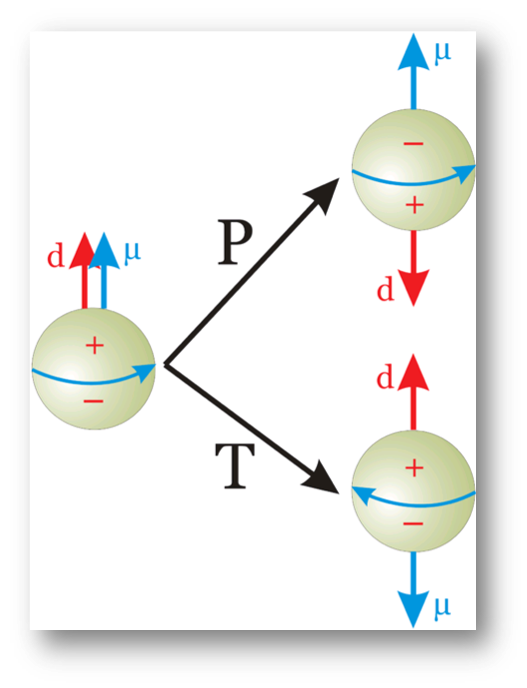
\includegraphics[width=1\textwidth]{EDM-graphic}
%     \end{figure}
% % \end{columns}

\end{frame}